\section{Experiments}
\label{sec:experiments}
\begin{figure*}
\centering
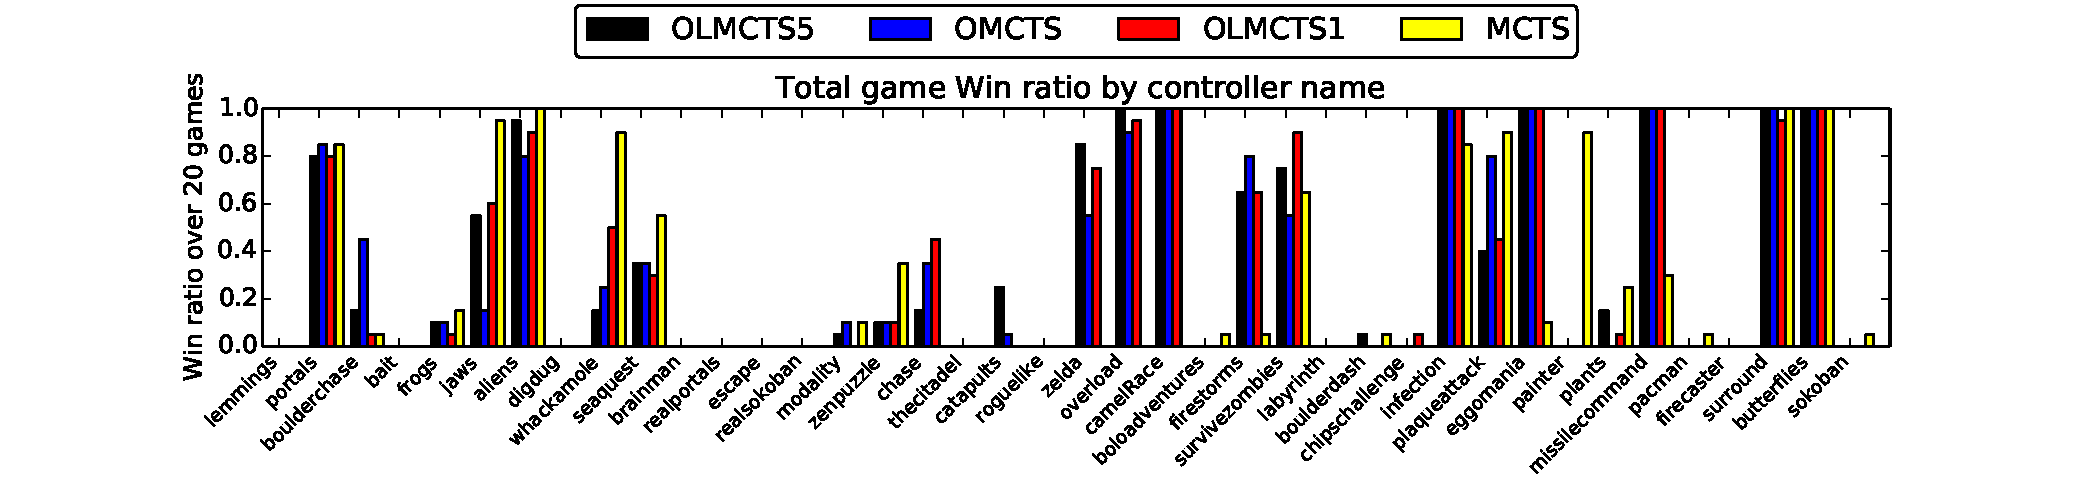
\includegraphics[width=\textwidth]{includes/wins}
%\vspace{-.4cm}
%\caption{Win ratio of the algorithms per game on all levels.}
%\label{fig:wins}
\centering
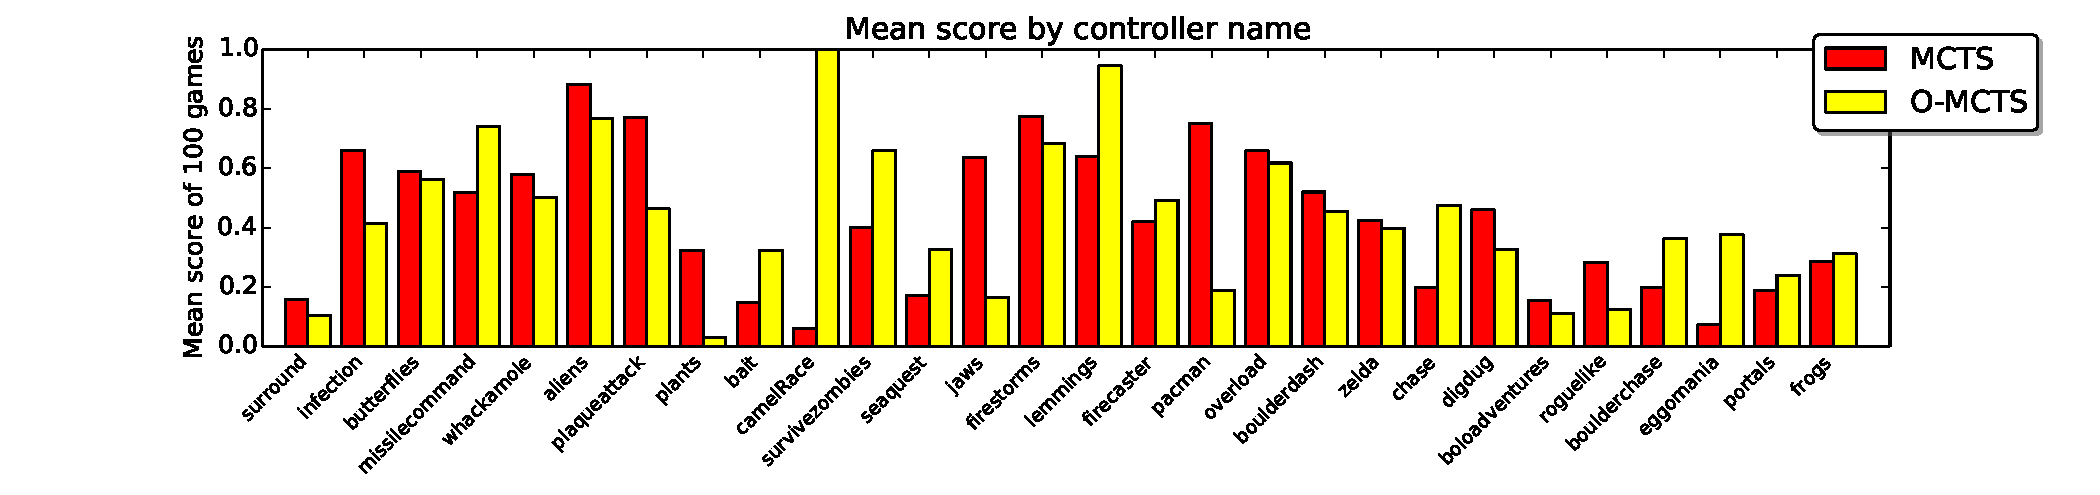
\includegraphics[width=\textwidth]{includes/scores}
\vspace{-.8cm}
\caption{Win ratio and mean normalized score of the algorithms per game. 1 means
the highest score achieved by all the algorithms, 0 the lowest.}
\label{fig:scores}
\end{figure*}

This section describes the experiments that have been done on
O-MCTS and OL-MCTS\@. The algorithms are compared to the MCTS
algorithm, as described in Section~\ref{subsec:mcts}. All algorithms are run on a set of
twenty-eight different games in the VGDL framework. The set consists of all the
games from the first four training sets of the GVGAI competition, excluding
puzzle games that can be solved by an exhaustive search and have no random
component (e.g. NPCs). Each game has five levels, the first of which
traditionally is the easiest and the last of which is the hardest.

Firstly, we compare O-MCTS to MCTS by showing the win ratio and mean score of
both algorithms on all the games. Secondly we show the improvement that OL-MCTS
makes compared to O-MCTS if it is allowed 4 games of learning time. We
demonstrate the progress it achieves by showing the first and last of the games
it plays.  Lastly we compare the three algorithms by summing over all the
victories of all the levels of each game.  Following the GVGAI competition's
scoring method, algorithms are primarily judged on their ability to win the
games. The scores they achieve are treated as a secondary objective.

For these experiments we construct an option set which is aimed at providing
action sequences for any type of game, since the aim here is general video game
playing. Note that a more specific set of options can be created when the
algorithm should be tailored to only one type of games and similarly: options
can be added and removed from the set easily.  The following options are
designed by us and used in the experiments of this paper.

\begin{itemize}[noitemsep]
	\item \texttt{ActionOption} executes a specific action once and then
		stops.
	\item \texttt{AvoidNearestNpcOption} makes the agent avoid the nearest NPC
	\item \texttt{GoNearMovableOption} makes the agent walk towards a
		movable game sprite (defined as movable by the VGDL) and stops when it
		is within a certain range of the movable
	\item \texttt{GoToMovableOption} makes the agent walk towards a
		movable until its location is the same as that of the movable
	\item \texttt{GoToNearestSpriteOfType} makes the agent walk to the nearest sprite of
		a specific type
	\item \texttt{GoToPositionOption} makes the agent walk to a specific position
	\item \texttt{WaitAndShootOption} waits until an NPC is in a specific location and
		then uses its weapon.
\end{itemize}

For each option type, a subtype per visible sprite type is created during the
game. For each sprite, an option instance of its corresponding subtype is
created. For example, the game \textit{zelda}, as seen in Figure~\ref{fig:zelda},
contains three different sprite types (excluding the avatar and walls);
monsters, a key and a portal. The first level contains three monsters, one key
and one portal. The aim of the game is to collect the key and walk towards
the portal without being killed by the monsters. The score is increased by 1 if
a monster is killed, i.e., its sprite is on the same location as the sword
sprite, if the key is picked up, or when the game is won.
\texttt{GoToMovableOption} and \texttt{GoNearMovableOptions} are created for
each of the three monsters and for the key. A \texttt{GoToPositionOption} is
created for the portal.  One \texttt{GoToNearestSpriteOfType} is created per
sprite type. One \texttt{WaitAndShootOption} is created for the monsters and
one \texttt{AvoidNearestNpc\-Option} is created. This set of options is $O$, as
defined in Section~\ref{subsec:options}. In a state where, for example, all the
monsters are dead, the possible option set $\mathbf{p}_s$ does not contain the
\texttt{AvoidNearestNpcOption} and \texttt{GoToMovableOption}s and
\texttt{GoNearMovableOption}s for the monsters.

The \texttt{GoTo\ldots} and \texttt{GoNear\ldots} options utilize an adaptation
of the A Star algorithm to plan their routes~\cite{hart1968formal}. An
adaptation is needed, because at the beginning of the game there is no knowledge
of which sprites are traversable by the avatar and which are not. Therefore,
during every move that is simulated by the agent, the A Star module has to
update its beliefs about the location of walls and other blocking objects. This
is accomplished by comparing the movement the avatar wanted to make to the
movement that was actually made in game. If the avatar did not move, it is
assumed that all the sprites on the location the avatar should have arrived in
are blocking sprites. A Star keeps a \emph{wall score} for each sprite type.
When a sprite blocks the avatar, its wall score is increased by one.
Additionally, when a sprite kills the avatar, its wall score is increased by
100, in order to prevent the avatar from walking into killing sprites.
Traditionally the A Star's heuristic uses the distance between two points. Our A
Star adaptation adds the wall score of the goal location to this heuristic,
encouraging the algorithm to take paths with a lower wall score. This method
enables A Star to try to traverse paths that were unavailable earlier, while
preferring safe and easily traversable paths. For example in \textit{zelda}, a
door is closed until a key is picked up. Our A Star version will still be able
to plan a path to the door once the key is picked up, winning the game.

We empirically optimize the parameters of the O(L)-MCTS algorithm
for these experiments. We use discount factor $\gamma = 0.9$, maximum action
time $t = 40$ milliseconds. The maximum search depth $d$ is set to 70, which is
higher than most alternative tree search algorithms, for example in the GVGAI
competition, use. The number of node visits after which \textsf{uct} is used,
$v$, is set to 40. Crazy stone parameter $K$ is set to $0.5$.  For comparison,
we use the MCTS algorithm provided with the Java implementation of VGDL with its
default value of maximum search depth of 10. Both algorithms have \textsf{uct}
constant $C_p = \sqrt{2}$. Unfortunately, comparing to Q-learning with options
was impossible, because the state space of these games is too big for the
algorithm to learn any reasonable behavior. All the experiments are run on an
Intel i7-2600, 3.40GHz quad core processor with 6 GB of DDR3, 1333 MHz RAM
memory. In all the following experiments on this game set, each algorithm plays
each of the 5 levels of every game 20 times. 

\subsection{O-MCTS}
\label{subsec:omcts}
This section describes the results of the option Monte Carlo tree search
algorithm in comparison with the standard Monte Carlo tree search algorithm.
This demonstrates the improvement that can be achieved by using our method to
enhance MCTS with our option set.
The games in this and the following experiments are ordered by the performance
an algorithm that always chooses a random action, indicating the complexity of
the games.  From left to right, the random algorithm's win ratio and score
decreases. Figure~\ref{fig:scores} shows the win ratio and normalized
score of the algorithms for each game. In short, the O-MCTS algorithms performs
at least as good as MCTS in almost all games, and better in most.

O-MCTS outperforms MCTS in the games \textit{missile command}, \textit{bait},
\textit{camel race}, \textit{survive zombies}, \textit{firestorms},
\textit{lemmings}, \textit{firecaster}, \textit{overload}, \textit{zelda},
\textit{chase}, \textit{boulderchase} and \textit{eggomania} winning more games
or achieving a higher mean score. By looking at the algorithm's actions for
these games, we can see that O-MCTS succeeds in efficiently planning paths in a
dangerous environment, enabling it to do a further forward search than the
ordinary Monte Carlo tree search. 
\textit{Camel race} requires the player to
move to the right for 80 consecutive turns to reach the finish line. No
intermediate rewards are given to indicate that the agent is walking in the
right direction. This is hard for MCTS, since it only looks 10 turns ahead.
O-MCTS always wins this game, since it can plan forward a lot further.
Furthermore, the rollouts of the option for walking towards the finish line have
a bigger chance of reaching the finish line than the random rollouts executed by
MCTS\@.
In \textit{Overload}, a sword has to be picked up before the avatar can finish the
game, which seems to be too hard for MCTS, but poses less of a problem for
O-MCTS\@.  Furthermore, in \textit{zelda} we can see that the MCTS algorithm
achieves roughly the same score as O-MCTS, but does not win the game, since
picking up the key and walking towards the door is a difficult action sequence.
We assume that the mean score achieved by MCTS is because it succeeds in killing
the monsters, whereas O-MCTS achieves its score by picking up the key and
walking to the door.  These results indicate that O-MCTS performs better than
MCTS in games where a sequence subgoals have to be reached.

The MCTS algorithm performs better than O-MCTS in \textit{pacman},
\textit{whackamole}, \textit{jaws}, \textit{seaquest} and \textit{plaque attack}
(note that for \textit{seaquest}, O-MCTS has a higher mean score, but wins less
than MCTS). A parallel between these games is that they have a very
big number of different sprites, for each of which several options have to be
created by O-MCTS\@. When the number of options becomes too big, constructing the
set of possible options $\mathbf{p}_s$ for every state $s$ becomes so
time-consuming that the algorithm has too little time to build a tree and find
the best possible action. To test this hypothesis we increased the computation
time for O-MCTS to 120ms and found that the win ratio of O-MCTS increases to
around $0.8$ for \textit{seaquest} and \textit{plaque attack}, whereas the win
ratio for MCTS increased to $0.9$ and $0.7$ respectively. This means that with
more action time, the difference between O-MCTS and MCTS is reduced for
\textit{seaquest} and O-MCTS outperforms MCTS on \textit{plaque attack}.

\begin{figure}
	\centering
	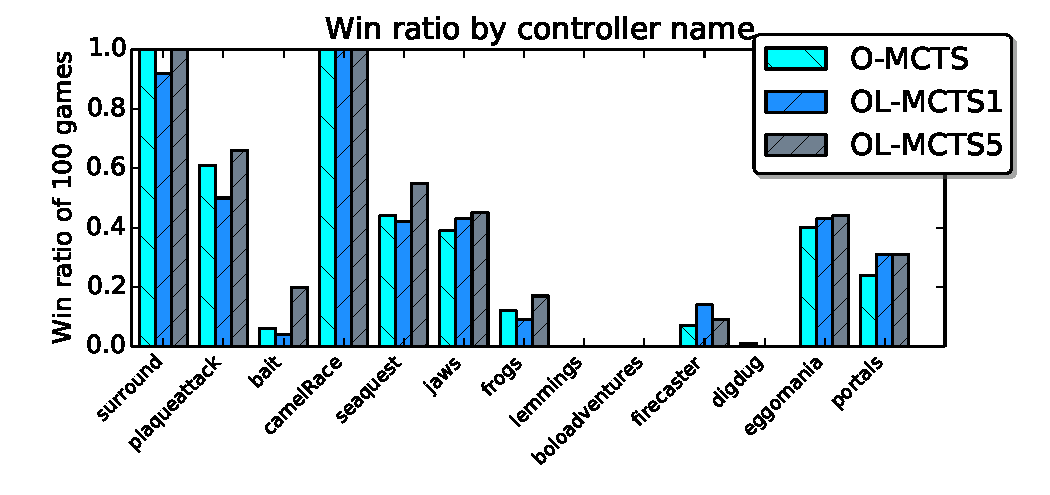
\includegraphics[width=\columnwidth]{includes/winsOLMCTS}
	%\vspace{-.8cm}
	%\caption{Win ratio comparison of OL-MCTS and O-MCTS.}
	%\label{fig:wins-olmcts}
	\centering
	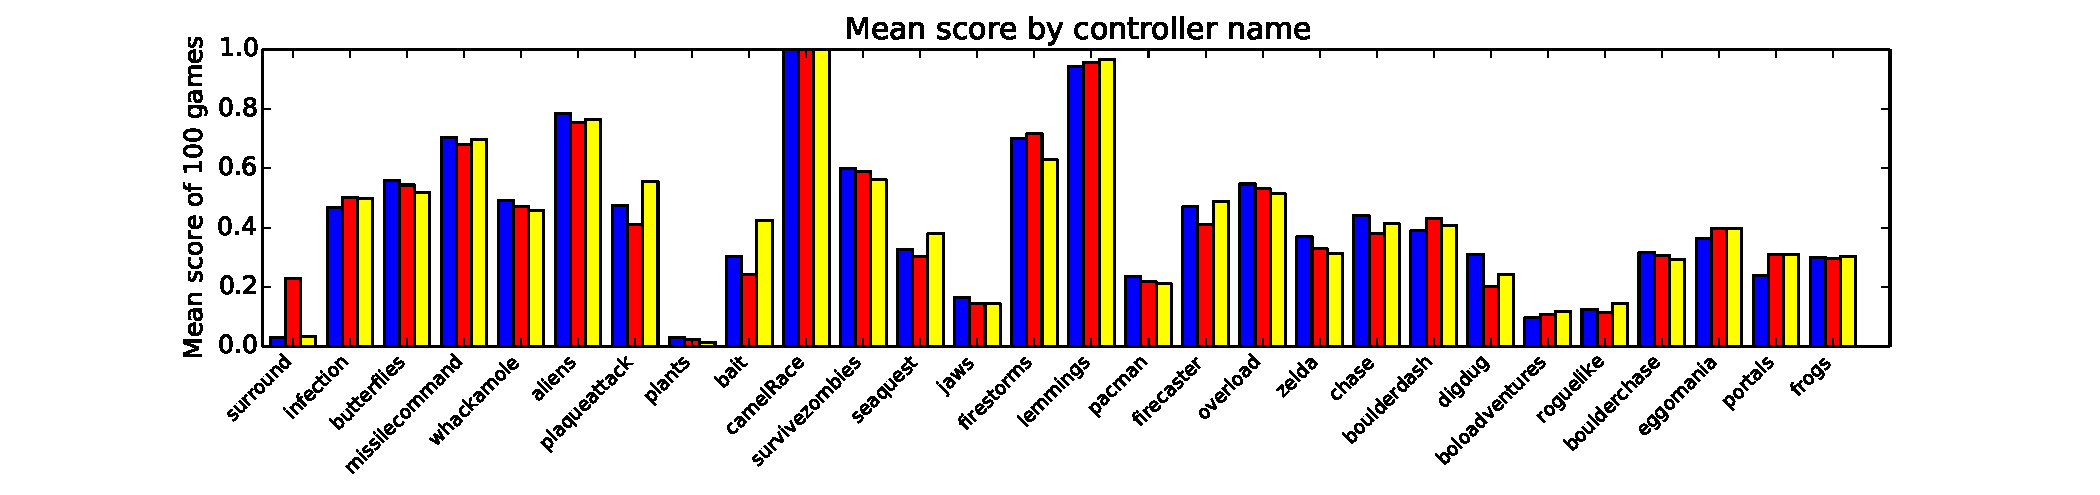
\includegraphics[width=\columnwidth]{includes/scoresOLMCTS}
	\vspace{-.8cm}
	\caption{Normalized win ratio and score comparison of OL-MCTS and O-MCTS\@.
	OL-MCTS outperforms O-MCTS by a small margin in some games. In the games
	that are not shown both algorithms perform equally.}
	\label{fig:scores-olmcts}
\end{figure}

\subsection{OL-MCTS}
\label{subsec:olmcts}
Secondly, we compare OL-MCTS to O-MCTS by running it on the same set of games.
The option learning algorithm is allowed four learning games, after which the
fifth is used for the comparisons. Figure~\ref{fig:scores-olmcts} shows the
performance difference between O-MCTS and OL-MCTS on some games. For the other
games, the performance was approximately the same. Here OL-MCTS1 shows the
performance of OL-MCTS on the first game. OL-MCTS5 shows the performance of the
algorithm after learning for four games. 

We can see that, although the first iteration of OL-MCTS sometimes performs a
bit worse than O-MCTS, the fifth iteration often scores at least as high, or
higher than O-MCTS\@. We expect that the loss of performance in OL-MCTS1 is
a result of the extra overhead that is added by the crazy stone algorithm: A
sorting of all the options has to take place in each tree node. The learning
algorithm significantly improves score and win ratio for the game \textit{bait},
which is a game in which the objective is to reach a goal portal after
collecting a key.  The player can push boxes around to open paths. There are
holes in the ground that kill the player unless they are filled with boxes,
which make both the hole and the box disappear. 
Figure~\ref{fig:learning-results} shows the improvement in score and win ratio
for this game. There are two likely explanations for this improvement: 1.) There
are sprites that kill the player, which are evaded by the algorithm when it has
learned to do so.  2.) The algorithm learns that it should pick up the key.

Furthermore, we can see small improvements on the games \textit{seaquest} and
\textit{jaws}, on which O-MCTS performs worse than MCTS\@.  Although OL-MCTS does
not exceed the score of the original Monte Carlo tree search algorithm, this
improvement suggests that OL-MCTS is on the right path of improving O-MCTS\@.

\begin{figure}
	\centering
	\subfigure[Learning \textit{bait}]{%
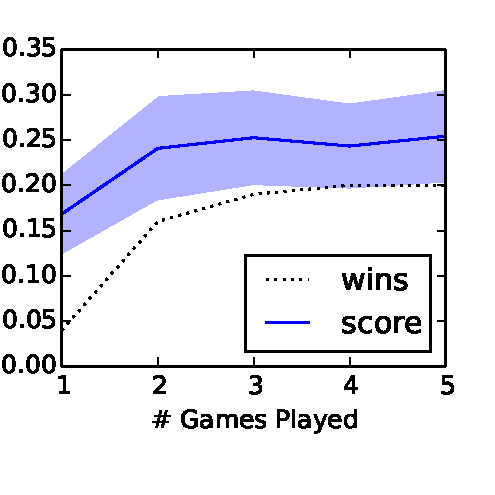
\includegraphics[scale=.44]{includes/learning}%
\label{fig:learning-results}%
	}
	\subfigure[Totals]{%
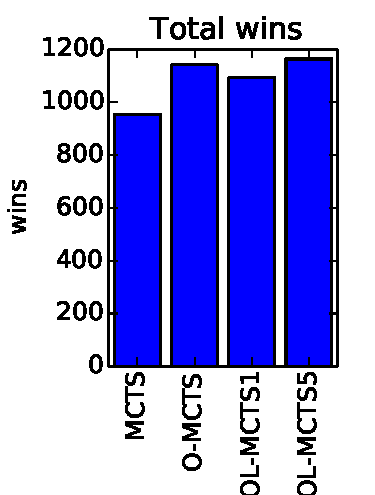
\includegraphics[scale=.44]{includes/totals.pdf}%
\label{fig:total-results}%
	}
	\caption{Learning improvement on game \textit{bait}, it shows win ratio and
		normalized score. Total number of wins of the algorithms on
	all games.}
\end{figure}

\subsection{Totals}
\label{subsec:totals}
Figure~\ref{fig:total-results} shows the sum of wins over all games, all levels.
It shows a significant ($p < 0.05$) improvement of O-MCTS and OL-MCTS over
MCTS\@.  There is no significant difference in performance of OL-MCTS over
O-MCTS, although our results suggest that it does improve for a subset of the
games. 

Summarizing, our tests indicate that on complex games O-MCTS outperforms MCTS\@.
For other games it performs at least as well, as long as the number of game
sprites is not too high.  The OL-MCTS algorithm can increase performance for
some of the games, such as \textit{bait} and \textit{plaque attack}. On other
games, little to no increased performance can be found.
